%%%%% Document Setup %%%%%%%%

\documentclass[12pt, onecolumn]{revtex4}    % Font size (12pt) and column number (one or two).

\usepackage[a4paper, left=2.5cm, right=2.5cm, top=2.5cm, bottom=2.5cm]{geometry}  % Defines paper size and margin length

\renewcommand{\baselinestretch}{1}     % Defines the line spacing

\usepackage{subcaption}

\usepackage[font=small, labelfont=bf]{caption}                      % Defines caption font size and caption title bolded
\captionsetup[figure]{justification=justified, singlelinecheck, font=small} 
\captionsetup[table]{justification=justified, singlelinecheck=off, font=small} 
\captionsetup{compatibility=false}

\usepackage{graphics,graphicx,epsfig,ulem}	% Makes sure all graphics works
\usepackage{amsmath} 						% Adds mathematical features for equations

\usepackage{fancyhdr}

\usepackage{textcomp}

\usepackage{tabularx}

\def\thesection{\arabic{section}}
\def\thesubsection{\alph{subsection}}

\def\bibsection{\section*{References}}        % Position reference section correctly

%%%%% Document %%%%%
\begin{document}                     

\title{Testing the Milankovitch-Croll hypothesis using $\delta^{18}$O foram data} 
\maketitle
%\thispagestyle{plain} % produces page number for front page

\vspace{-4ex}

The Milankovitch-Croll hypothesis suggests that changes in the Earth's orbit around the Sun leads to changes in the Earth's planetary climate through fluctuations in solar insolation \cite{ruddiman_climate}. The exploration of this hypothesis can be performed by analysing proxy data, deep ocean sediment cores, paired together with Earth orbital data. Sediment cores provide a way to show the global temperature fluctuations and global ice volue across Earth's history. They contain a trace, namely the $\delta^{18}$O ratio in foram shells \cite{droxler_climate}. \\

Defined from laboratory experiments, a $\sim 5^{\circ}\mathrm{C}$ temperature increase leads to an $\sim 1$\textperthousand\ decrease in the $\delta^{18}$O ratio. As ice-sheets melt, more $^{16}$O is released into the oceans, thus reducing the ratio. Sediment core data for an early and late period of Earth's history (Fig.~\ref{fig:foram_data}) shows that in the more recent age the temperature had been shifting more dramatically as the amplitude of the $\delta^{18}$O had been varying more considerably than from 4 Myr to 5 Myr BP. This would have lead to longer periods of cooling and with a cooler climate, there would be a larger amount of global ice. In both sets of $\delta^{18}$O data, there features a sinusoidal-like trend, albeit the historical data has a smaller amplitude. This suggests that the glacial-interglacial events are a normal part of Earth's planetary climate cycle and could be related to the cyclical Earth-Sun orbital relationship. \\

In looking at the astrophysical data there are three concepts to consider: (i) eccentricity, (ii) precession, and (iii) obliquity. The former describes the ellipticity of the Earth's orbit around the Sun \cite{carroll_astro}, it's effect on insolation however is not entirely independent as the eccentricity also depends on the orbital angle between the solstices and the position of perihelion/aphelion. A precessional index value can be produced with $\chi= \varepsilon \sin{\omega}$, where $\varepsilon$ is the eccentricity and $\omega$ is the angle. Finally the obliquity can be defined as the value which describes the degree of tilt of the Earth's axis. \\

With these definitions in mind, we can proceed to evaluate and verify that our orbital data agrees with literature by applying two statistical analysis techniques. The first tool is \textit{wavelet transform} (WT) analysis, by using the WT tool in PAST3 \cite{past3} heatmaps (Fig.~\ref{fig:wa_orbital_data}) can be obtained which contain the dominant frequencies from a dataset. The second technique to employ is \textit{REDFIT} analysis, frequencies (Fig.~\ref{fig:d18o_redfit}) can be picked out by finding peaks which have a height greater than a $95\%$ confidence interval. \\

Processing the orbital data with these two tools we can obtain results (Table \ref{table:final_results}) which have an average $\sim 96 \%$ agreement when compared with literature wavelengths. Knowing that the methods are valid and that they produce accurate results, the $\delta^{18}$O foram data can be analysed using the same tools. \\

There is a signal which can be attributed to the obliquity as wavelengths of 41.1 ka (REDFIT) and 38.9 ka (WT) are comparable to the actual value 41 ka. However from the WT analysis (Fig.~\ref{fig:wa_d18o}) this signal is only prevalent from 0.15 Myr to 1.28 Myr BP even if it is the strongest (hottest). There is a complete disconnect which could be attributed to the rise of an eccentricity signal of 96.0 ka which spans from $\sim 1.28$ Myr to 4.80 Myr BP. A similar wavelength of 96.3 ka can be found from REDFIT, both together suggest that another orbital periodicity feature is evident in the $\delta^{18}$O data. It is therefore not unreasonable to search for a perihelion longitude wavelength, consequently one signal is apparent but it can only be seen with REDFIT analysis, 23.7 ka. The lack of this signal in WT could be attributed to the fact that the data is dominated by much stronger features, and even with the REDFIT fitting (Fig.~\ref{fig:d18o_redfit}) it can be seen that this perihelion signal is weak compared to the other two peaks. \\

It can be suggested that the Milankovitch-Croll hypothesis has some merit as the results do agree. The issue arises is \\

\newpage

%\twocolumngrid

\bibliographystyle{unsrt}
\bibliography{practical_2}

\newpage

\section*{Appendices}
\begin{figure}[!h]
\begin{center}
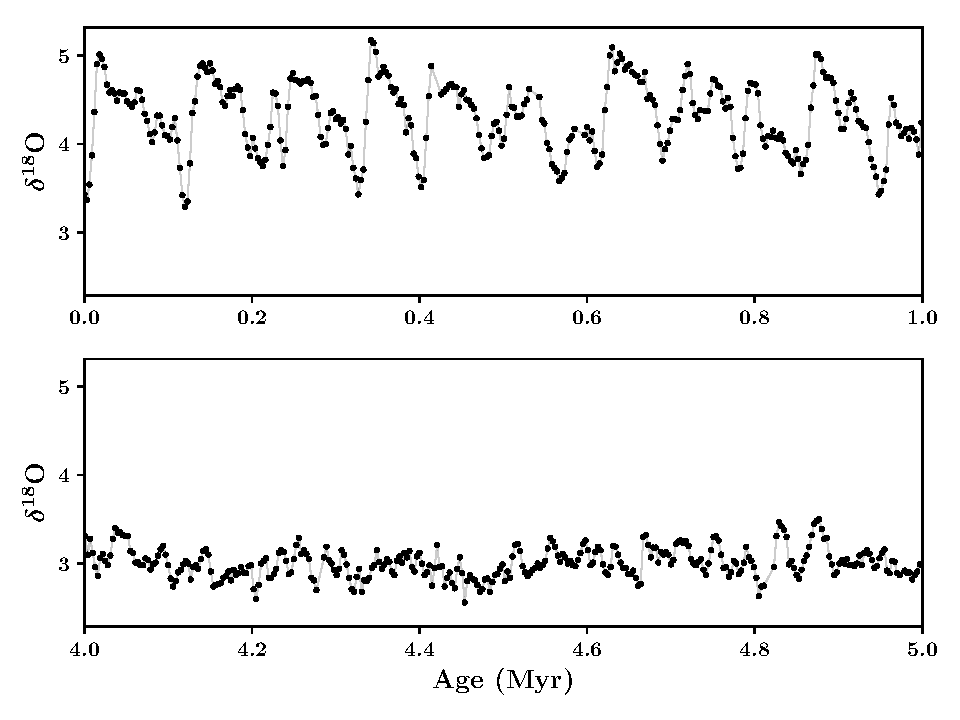
\includegraphics[width=11cm]{figures/foram_data}
\caption[]{Plots of the marine benthic foram $\delta^{18}$O data against age, with increasing time to the right. Both data sets have been taken out of a larger set which spans from 0 Myr to 6 Myr. As we move closer towards the present day, the periodicity and amplitude is larger which implies more extreme temperature variations so longer glacial-interglacials and a larger change in the global ice volume.}
\vspace{-3ex}
\label{fig:foram_data}
\end{center}
\end{figure}

\begin{figure}[!h]
\begin{center}
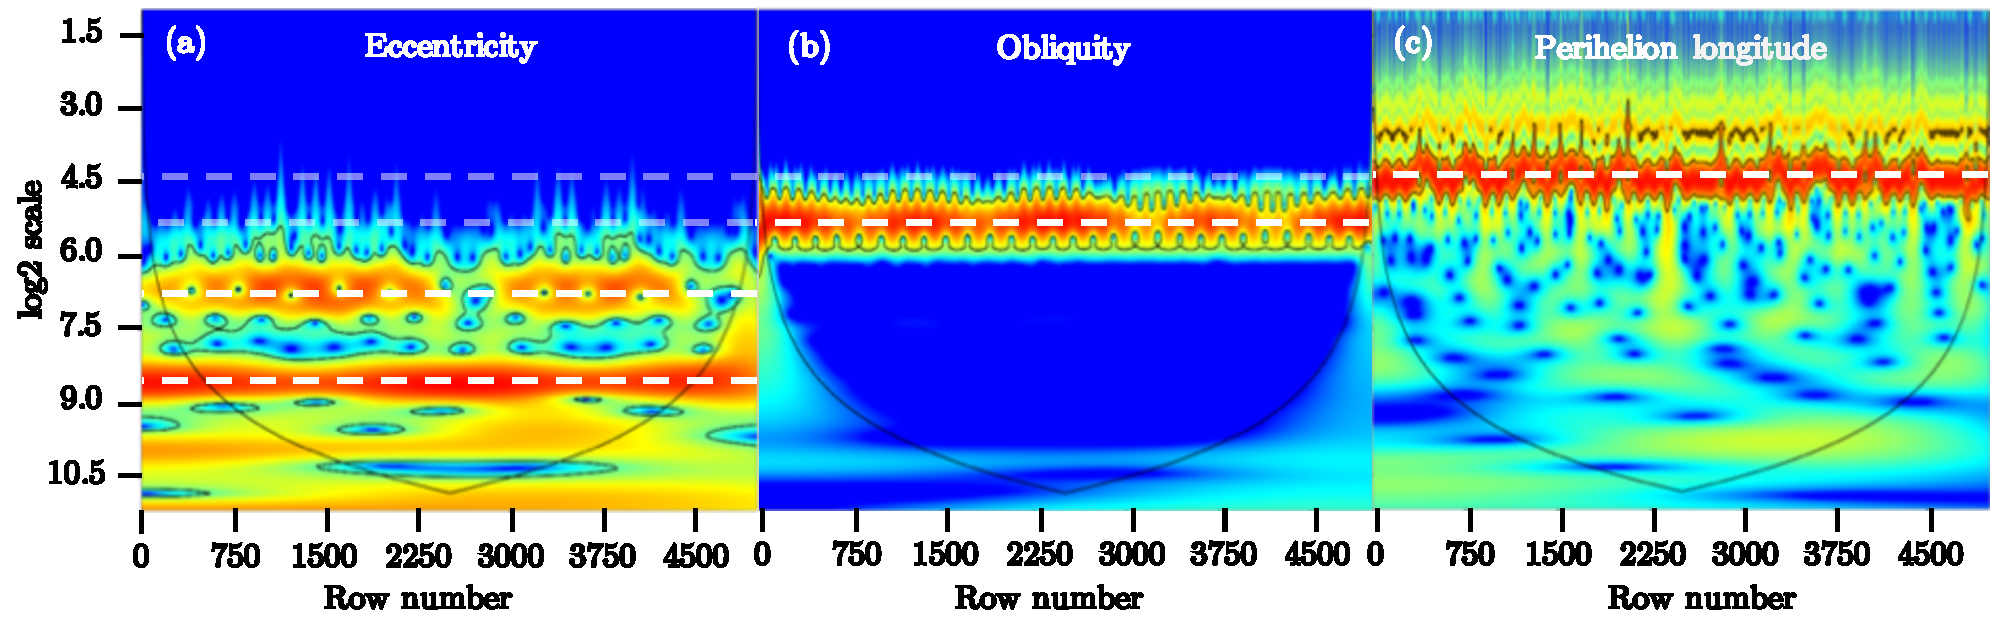
\includegraphics[width=16cm]{figures/wa_orbital_data}
\caption[]{The eccentricity, obliquity and perihelion longitude (precession) orbital data which has been processed with the wavelet transform analysis tool in PAST3. The periodicities from the data can be obtained by considering the ``hottest'' areas of each of the heat maps (i.e. the red/orange areas). Values for the wavelength can be found with $2^y \times P$, where $y$ is the y-axis height of the hot region, and $P$ is the period of time between the data points. In Table \ref{table:final_results} we summarise the wavelengths which correspond to the dashed-line heights.}
\vspace{-3ex}
\label{fig:wa_orbital_data}
\end{center}
\end{figure}

\begin{figure}[!h]
\begin{center}
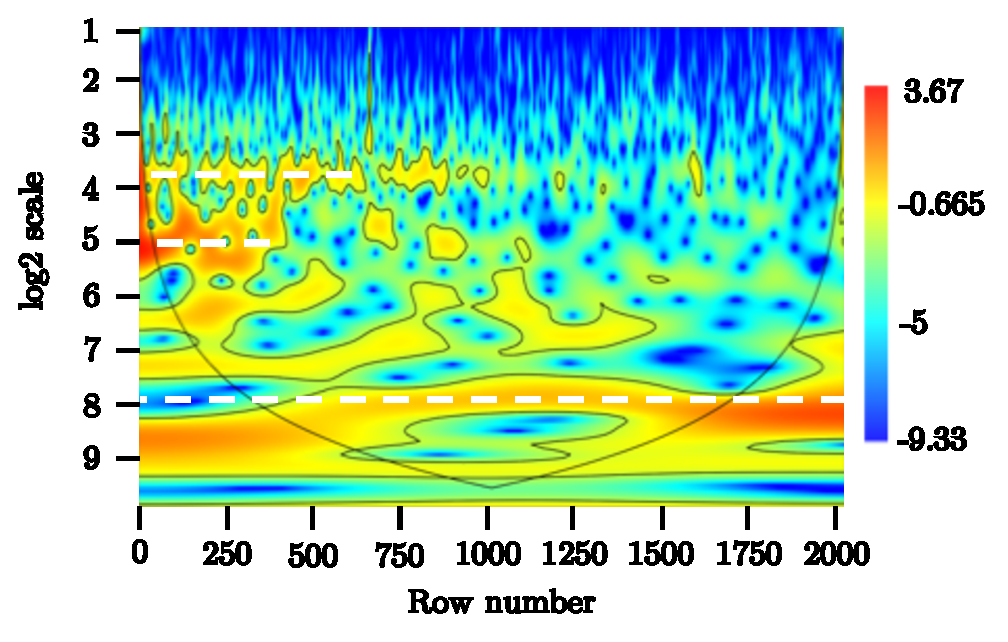
\includegraphics[width=11cm]{figures/wa_d18O.pdf}
\caption[]{The result from applying the PAST3 wavelet transform analysis tool to the $\delta^{18}$O benthic foram data, the wavelengths found are summarised in Table \ref{table:final_results}. The results are similar to those found in the orbital data, which could imply that orbital forcing does have an influence on glacial-interglacial climate.}
\vspace{-3ex}
\label{fig:wa_d18o}
\end{center}
\end{figure}

\begin{figure}[!h]
\begin{center}
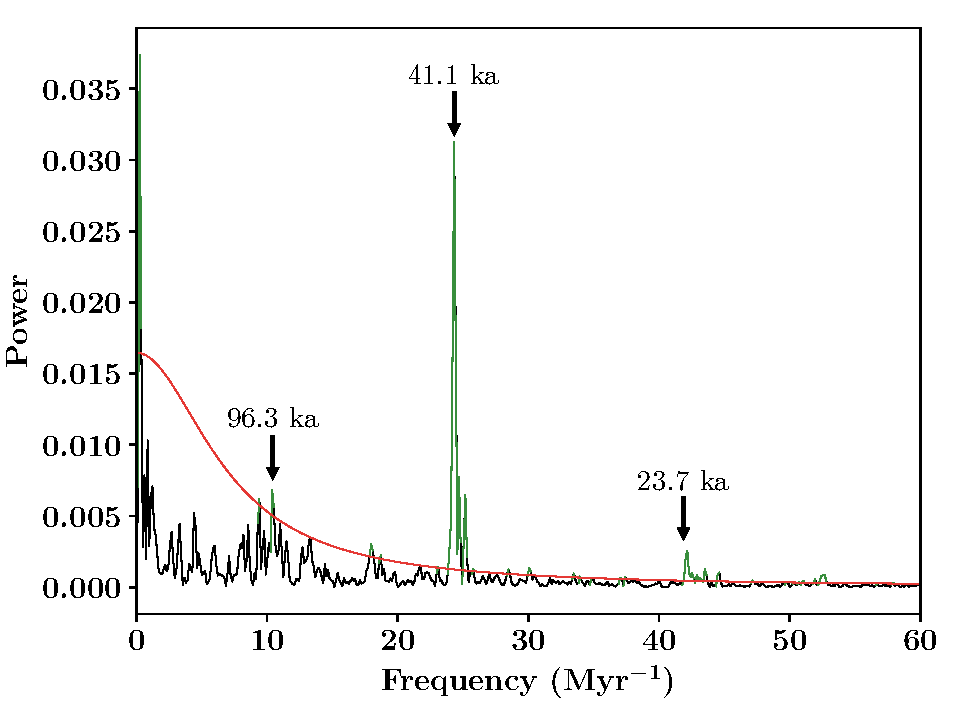
\includegraphics[width=11cm]{figures/d18O_redfit}
\caption[]{The benthic foram $\delta^{18}$O data analysed using the REDFIT spectral analysis tool in PAST3. Three dominant signals can be seen as coloured in green, they are defined as the main signals as they have a height greater than the $95\%$ confidence interval (the red curve). The same results can be found in Table \ref{table:final_results}, and comparing to the ``true'' wavelengths we also find similarities which further strengthens the possibility that the Milankovitch-Croll hypothesis has some validity.}
\vspace{-3ex}
\label{fig:d18o_redfit}
\end{center}
\end{figure}

\begin{table}[h!]
\centering
\begin{tabular}{c@{\hskip 20pt}c@{\hskip 20pt}c@{\hskip 20pt}c} 
 \hline
  & \textbf{Literature (ka)} &\textbf{REDFIT (ka)} & \textbf{WT (ka)} \\ [0.5ex] 
 Eccentricity & 100, 413 & 95.2, 128.2, 416.7 & 89.1, 100.4,  401.7\\
 Perihelion Longitude & 23, 100 & 23.8, 22.2 & 21.1 \\
 Obliquity & 41 & 41.7 & 39.4 \\
 $\delta^{18}$O & & 23.7, 41.1, 96.3  & 38.9, 96.0, 271.5, \\
 & & & 945.5, 1247.6 \\
 \hline
\end{tabular}
\caption{Table showing different sets of wavelength data: the approximate correct wavelengths for the periodicity of the orbital features \cite{campisano_milankovitch}, the results of the REDFIT spectral analysis and Wavelet Transform (WT) analysis on the orbital and benthic foram data. We find that as tools both REDFIT and WT are able to obtain similar periodicities which then agree with the literature values. }
\vspace{-0.5em}
\label{table:final_results}
\end{table}

\end{document}